\documentclass[12pt, titlepage]{article}

\usepackage{fullpage}
\usepackage[round]{natbib}
\usepackage{multirow}
\usepackage{booktabs}
\usepackage{tabularx}
\usepackage{graphicx}
\usepackage{float}
\usepackage{hyperref}
\hypersetup{
    colorlinks,
    citecolor=blue,
    filecolor=black,
    linkcolor=red,
    urlcolor=blue
}

\input{../../Comments}
%% Common Parts

\newcommand{\progname}{Software Engineering} % PUT YOUR PROGRAM NAME HERE
\newcommand{\authname}{Team \#2, Team Name
\\ Zihao Du 
\\ Matthew Miller
\\ Firas Elayan
\\ Abhiram Neelamraju
\\ Michael Kim} % AUTHOR NAMES                  

\usepackage{hyperref}
    \hypersetup{colorlinks=true, linkcolor=blue, citecolor=blue, filecolor=blue,
                urlcolor=blue, unicode=false}
    \urlstyle{same}
                                


\newcounter{acnum}
\newcommand{\actheacnum}{AC\theacnum}
\newcommand{\acref}[1]{AC\ref{#1}}

\newcounter{ucnum}
\newcommand{\uctheucnum}{UC\theucnum}
\newcommand{\uref}[1]{UC\ref{#1}}

\newcounter{mnum}
\newcommand{\mthemnum}{M\themnum}
\newcommand{\mref}[1]{M\ref{#1}}

\begin{document}

\title{Module Guide for \progname{}} 
\author{\authname}
\date{\today}

\maketitle

\pagenumbering{roman}

\section{Revision History}

\begin{tabularx}{\textwidth}{p{3cm}p{2cm}X}
\toprule {\bf Date} & {\bf Version} & {\bf Notes}\\
\midrule
Jan 11 & 1.0 & Add Section Timeline and Reflection\\
Jan 15 & 1.0 & Revision 0\\
\bottomrule
\end{tabularx}

\newpage

\section{Reference Material}

This section records information for easy reference.

\subsection{Abbreviations and Acronyms}

\renewcommand{\arraystretch}{1.2}
\begin{tabular}{l l} 
  \toprule		
  \textbf{symbol} & \textbf{description}\\
  \midrule 
  AC & Anticipated Change\\
  DAG & Directed Acyclic Graph \\
  M & Module \\
  MG & Module Guide \\
  OS & Operating System \\
  R & Requirement\\
  SC & Scientific Computing \\
  SRS & Software Requirements Specification\\
  \progname & Explanation of program name\\
  UC & Unlikely Change \\
  CRUD & Create, Read, Update and Delete\\
  \bottomrule
\end{tabular}\\

\newpage

\tableofcontents

\listoftables

\listoffigures

\newpage

\pagenumbering{arabic}

\section{Introduction}

Decomposing a system into modules is a commonly accepted approach to developing
software.  A module is a work assignment for a programmer or programming
team~\citep{ParnasEtAl1984}.  We advocate a decomposition
based on the principle of information hiding~\citep{Parnas1972a}.  This
principle supports design for change, because the ``secrets'' that each module
hides represent likely future changes.  Design for change is valuable in SC,
where modifications are frequent, especially during initial development as the
solution space is explored.  

Our design follows the rules layed out by \citet{ParnasEtAl1984}, as follows:
\begin{itemize}
\item System details that are likely to change independently should be the
  secrets of separate modules.
\item Each data structure is implemented in only one module.
\item Any other program that requires information stored in a module's data
  structures must obtain it by calling access programs belonging to that module.
\end{itemize}

After completing the first stage of the design, the Software Requirements
Specification (SRS), the Module Guide (MG) is developed~\citep{ParnasEtAl1984}. The MG
specifies the modular structure of the system and is intended to allow both
designers and maintainers to easily identify the parts of the software.  The
potential readers of this document are as follows:

\begin{itemize}
\item New project members: This document can be a guide for a new project member
  to easily understand the overall structure and quickly find the
  relevant modules they are searching for.
\item Maintainers: The hierarchical structure of the module guide improves the
  maintainers' understanding when they need to make changes to the system. It is
  important for a maintainer to update the relevant sections of the document
  after changes have been made.
\item Designers: Once the module guide has been written, it can be used to
  check for consistency, feasibility, and flexibility. Designers can verify the
  system in various ways, such as consistency among modules, feasibility of the
  decomposition, and flexibility of the design.
\end{itemize}

The rest of the document is organized as follows. Section
\ref{SecChange} lists the anticipated and unlikely changes of the software
requirements. Section \ref{SecMH} summarizes the module decomposition that
was constructed according to the likely changes. Section \ref{SecConnection}
specifies the connections between the software requirements and the
modules. Section \ref{SecMD} gives a detailed description of the
modules. Section \ref{SecTM} includes two traceability matrices. One checks
the completeness of the design against the requirements provided in the SRS. The
other shows the relation between anticipated changes and the modules. Section
\ref{SecUse} describes the use relation between modules.

\section{Anticipated and Unlikely Changes} \label{SecChange}

This section lists possible changes to the system. According to the likeliness
of the change, the possible changes are classified into two
categories. Anticipated changes are listed in Section \ref{SecAchange}, and
unlikely changes are listed in Section \ref{SecUchange}.

\subsection{Anticipated Changes} \label{SecAchange}

Anticipated changes are the source of the information that is to be hidden
inside the modules. Ideally, changing one of the anticipated changes will only
require changing the one module that hides the associated decision. The approach
adapted here is called design for
change.

\begin{description}
\item[\refstepcounter{acnum} \actheacnum \label{acHardware}:] The specific
  hardware on which the software is running.
\item[\refstepcounter{acnum} \actheacnum \label{acInput}:] The format of the
  initial input data.
\item ...
\end{description}

\subsection{Unlikely Changes} \label{SecUchange}

The module design should be as general as possible. However, a general system is
more complex. Sometimes this complexity is not necessary. Fixing some design
decisions at the system architecture stage can simplify the software design. If
these decision should later need to be changed, then many parts of the design
will potentially need to be modified. Hence, it is not intended that these
decisions will be changed.

\begin{description}
\item[\refstepcounter{ucnum} \uctheucnum \label{ucIO}:] Input/Output devices
  (Input: File and/or Keyboard, Output: File, Memory, and/or Screen).
\item ...
\end{description}

\section{Module Hierarchy} \label{SecMH}

This section provides an overview of the module design. Modules are summarized
in a hierarchy decomposed by secrets in Table \ref{TblMH}. The modules listed
below, which are leaves in the hierarchy tree, are the modules that will
actually be implemented.

\begin{description}
\item [\refstepcounter{mnum} \mthemnum \label{mHH}:] Hardware-Hiding Module
\item [\refstepcounter{mnum} \mthemnum \label{mDB}:] Database Module
\item [\refstepcounter{mnum} \mthemnum \label{mServer}:] Server Module
\item [\refstepcounter{mnum} \mthemnum \label{mAuth}:] Authentication Module
\item [\refstepcounter{mnum} \mthemnum \label{mARCamera}:] AR Camera Module
\item [\refstepcounter{mnum} \mthemnum \label{mARInterface}:] AR Interface Module
\item [\refstepcounter{mnum} \mthemnum \label{mMap}:] Map Module
\item [\refstepcounter{mnum} \mthemnum \label{mUser}:] User Module
\item [\refstepcounter{mnum} \mthemnum \label{mLec}:] Lecture Module
\item [\refstepcounter{mnum} \mthemnum \label{mEvent}:] Event Module
\item [\refstepcounter{mnum} \mthemnum \label{mUP}:] User Profile Module
\item [\refstepcounter{mnum} \mthemnum \label{mFM}:] Friend Manager Module
\item [\refstepcounter{mnum} \mthemnum \label{mADV}:] Activity Detail View Module
\item [\refstepcounter{mnum} \mthemnum \label{mLDV}:] Lecture Detail View Module
\item [\refstepcounter{mnum} \mthemnum \label{mEDV}:] Event Detail View Module
\item [\refstepcounter{mnum} \mthemnum \label{mPF}:] Pagination and Filter Module
\item [\refstepcounter{mnum} \mthemnum \label{mLL}:] Lecture List Manager Module
\item [\refstepcounter{mnum} \mthemnum \label{mEL}:] Event List Manager Module
\item [\refstepcounter{mnum} \mthemnum \label{mNotify}:] Notification Module
\end{description}


\begin{table}[h!]
\centering
\begin{tabular}{p{0.3\textwidth} p{0.6\textwidth}}
\toprule
\textbf{Level 1} & \textbf{Level 2}\\
\midrule

{Hardware-Hiding Module} & ~ \\
\midrule

\multirow{7}{0.3\textwidth}{Behaviour-Hiding Module}
& AR Interface\\
& User Module\\
& Lecture Module\\
& Event Module\\
& User Profile Module\\
& Friend Manager Module\\ 
& Lecture Detail View Module\\
& Event Detail View Module\\
& Lecture List Manager Module\\
& Event List Manager Module\\
& Notification Module\\
\midrule

\multirow{3}{0.3\textwidth}{Software Decision Module}
& Database Module\\
& Server Module\\
& Authentication Module\\
& AR Camera Module\\
& Map Module\\
& Activity Detail View Module\\
& Pagination and Filter Module\\
\bottomrule

\end{tabular}
\caption{Module Hierarchy}
\label{TblMH}
\end{table}

\section{Connection Between Requirements and Design} \label{SecConnection}

The design of the system is intended to satisfy the requirements developed in
the SRS. In this stage, the system is decomposed into modules. The connection
between requirements and modules is listed in Table~\ref{TblFRT}, \ref{TblNFRT}, \ref{TblNFRT-CONT}.

\section{Module Decomposition} \label{SecMD}

Modules are decomposed according to the principle of ``information hiding''
proposed by \citet{ParnasEtAl1984}. The \emph{Secrets} field in a module
decomposition is a brief statement of the design decision hidden by the
module. The \emph{Services} field specifies \emph{what} the module will do
without documenting \emph{how} to do it. For each module, a suggestion for the
implementing software is given under the \emph{Implemented By} title. If the
entry is \emph{OS}, this means that the module is provided by the operating
system or by standard programming language libraries.  \emph{\progname{}} means the
module will be implemented by the \progname{} software.

Only the leaf modules in the hierarchy have to be implemented. If a dash
(\emph{--}) is shown, this means that the module is not a leaf and will not have
to be implemented.

\subsection{Hardware Hiding Modules (\mref{mHH})}

\begin{description}
\item[Secrets:]The data structure and algorithm used to implement the virtual
  hardware.
\item[Services:]Serves as a virtual hardware used by the rest of the
  system. This module provides the interface between the hardware and the
  software. So, the system can use it to display outputs or to accept inputs.
\item[Implemented By:] OS
\end{description}

\subsection{Behaviour-Hiding Module}

\begin{description}
\item[Secrets:]The contents of the required behaviours.
\item[Services:]Includes programs that provide externally visible behaviour of
  the system as specified in the software requirements specification (SRS)
  documents. This module serves as a communication layer between the
  hardware-hiding module and the software decision module. The programs in this
  module will need to change if there are changes in the SRS.
\item[Implemented By:] --
\end{description}

\subsubsection{AR Interface Module (\mref{mARInterface})}
\begin{description}
\item[Secrets:]How AR User Interface elements are created and managed.
\item[Services:]Creates 3D AR elements when notified by the AR Camera of a new valid target. Handles user input relating to AR UI elements.
\item[Implemented By:] CampusConnections
\item[Type of Module:] Library
\end{description}

\subsubsection{Map Module (\mref{mMap})}
\begin{description}
\item[Secrets:]How users, events and buildings are organized and displayed on a virtual map.
\item[Services:]Displays points of interest such as buildings or events. Handles user interaction with points of interest. Displays user's avatar at their current location.
\item[Implemented By:] CampusConnections
\item[Type of Module:] Library
\end{description}

\subsubsection{Friend Manager Module (\mref{mFM})}

\begin{description}
\item[Secrets:]Friend related handlers including adding, deleting, messaging and viewing.
\item[Services:]Provides adding friend, deleting friend, message friend, view friend profile functionalities for the current user and displays friends and friend requests as lists.
\item[Implemented By:] CampusConnections
\item[Type of Module:] Library
\end{description}

\subsubsection{Lecture Detail View Module (\mref{mLDV})}

\begin{description}
\item[Secrets:]Module for editing user's lectures. Concrete class of Activity Detail View Module (\mref{mADV}).
\item[Services:]Provides functionality allowing users to view, add, edit, and delete lectures.
\item[Implemented By:] CampusConnections
\item[Type of Module:] Library
\end{description}

\subsubsection{Event Detail View Module (\mref{mEDV})}

\begin{description}
\item[Secrets:]Module for editing user's events. Concrete class of Activity Detail View Module (\mref{mADV}).
\item[Services:]Provides functionality allowing users to view, add, edit, and delete events.
\item[Implemented By:] CampusConnections
\item[Type of Module:] Library
\end{description}

\subsubsection{Notification Module (\mref{mNotify})}

\begin{description}
\item[Secrets:]Implementation detail and settings of toast notifications and alerts
\item[Services:]Provides functionalities to display all notifications, alerts and consents.
\item[Implemented By:] CampusConnections
\item[Type of Module:] Library
\end{description}

\subsubsection{Etc.}


\subsection{Software Decision Module}

\subsubsection{Database Module (\mref{mDB})}
\begin{description}
\item[Secrets:]Data structures of stored data and how database connection is established
\item[Services:]Provides CURD operations to database tables
\item[Implemented By:] Firebase, CampusConnections
\item[Type of Module:] Library
\end{description}

\subsubsection{Server Module (\mref{mServer})}
\begin{description}
\item[Secrets:]How data is sent to and received from clients.
\item[Services:]Provides real-time communication endpoints for chatting and location sharing.
\item[Implemented By:] CampusConnections
\item[Type of Module:] Library
\end{description}

\subsubsection{AR Camera Module (\mref{mARCamera})}
\begin{description}
\item[Secrets:]How AR targets are detected.
\item[Services:]Detects valid AR targets in the device's camera view and notifies the AR Interface module of the newly detected target.
\item[Implemented By:] Vuforia
\item[Type of Module:] Library
\end{description}

\subsubsection{Activity Detail View Module (\mref{mADV})}
\begin{description}
  \item[Secrets:]Abstract class for lectures/events.
  \item[Services:]Provides functionality for the Lecture/Event page, allowing the user to view, add, edit, and delete activities.
  \item[Implemented By:] Firebase, CampusConnections
  \item[Type of Module:] Library
  \end{description}

\subsubsection{Etc.}

\section{Traceability Matrix} \label{SecTM}

This section shows two traceability matrices: between the modules and the
requirements and between the modules and the anticipated changes.

% the table should use mref, the requirements should be named, use something
% like fref
\begin{table}[H]
\centering
\begin{tabular}{p{0.2\textwidth} p{0.6\textwidth}}
\toprule
\textbf{Req.} & \textbf{Modules}\\
\midrule
FR1-1 & \mref{mNotify}\\
FR2-1 & \mref{mAuth}, \mref{mDB}\\
FR2-2 & \mref{mAuth}, \mref{mUser}, \mref{mDB}\\
FR2-3 & \mref{mAuth}\\
FR2-4 & \mref{mAuth}\\
FR2-5 & \mref{mAuth}\\
FR2-6 & \mref{mUser}, \mref{mUP}, \mref{mDB}\\
FR2-7 & \mref{mAuth}, \mref{mUP}\\
FR2-8 & \mref{mUser}, \mref{mUP}, \mref{mDB}\\
FR3-1 & \mref{mFM}, \mref{mDB}\\
FR3-2 & \mref{mFM}, \mref{mDB}\\
FR3-3 & \mref{mFM}, \mref{mServer}\\
FR3-4 & \mref{mFM}, \mref{mServer}, \mref{mEvent}\\
FR3-5 & \mref{mFM}, \mref{mServer}, \mref{mMap}\\
FR3-6 & \mref{mFM}, \mref{mDB}\\
FR4-1 & \mref{mUP}, \mref{mDB}, \mref{mEvent}, \mref{mEDV}, \mref{mADV}\\
FR4-2 & \mref{mUP}, \mref{mDB}, \mref{mLec}, \mref{mLDV}, \mref{mADV}\\
FR4-3 & \mref{mEvent}, \mref{mEDV}, \mref{mADV}, \mref{mDB}, \mref{mAuth}\\
FR4-4 & \mref{mLec}, \mref{mLDV}, \mref{mADV}, \mref{mDB}, \mref{mAuth}\\
FR4-5 & \mref{mEvent}\\
FR4-6 & \mref{mLec}\\
FR4-7 & \mref{mEvent}, \mref{mEL}, \mref{mPF}\\
FR4-8 & \mref{mLec}, \mref{mLL}, \mref{mPF}\\
FR5-1 & \mref{mARCamera}\\
FR5-2 & \mref{mARInterface}\\
FR6-1 & \mref{mMap}, \mref{mDB}\\
FR6-2 & \mref{mMap}, \mref{mDB}\\
FR6-3 & \mref{mMap}, \mref{mServer}\\
\bottomrule
\end{tabular}
\caption{Trace Between Functional Requirements and Modules}
\label{TblFRT}
\end{table}

\begin{table}[H]
\centering
\begin{tabular}{p{0.2\textwidth} p{0.6\textwidth}}
\toprule
\textbf{Req.} & \textbf{Modules}\\
\midrule
LF-A1 & \mref{mARInterface} \mref{mFM}, \mref{mUP}, \mref{mLDV}, \mref{mEDV}, \mref{mLL}, \mref{mEL}, \mref{mNotify}\\
LF-A2 & \mref{mARInterface} \mref{mFM}, \mref{mUP}, \mref{mLDV}, \mref{mEDV}, \mref{mLL}, \mref{mEL}, \mref{mNotify}\\
LF-S1 & \mref{mARInterface} \mref{mFM}, \mref{mUP}, \mref{mLDV}, \mref{mEDV}, \mref{mLL}, \mref{mEL}, \mref{mNotify}\\
LF-S2 & \mref{mARInterface} \mref{mFM}, \mref{mUP}, \mref{mLDV}, \mref{mEDV}, \mref{mLL}, \mref{mEL}, \mref{mNotify}\\
UH-EOU1 & \mref{mARInterface} \mref{mFM}, \mref{mUP}, \mref{mLDV}, \mref{mEDV}, \mref{mLL}, \mref{mEL}, \mref{mNotify}\\
UH-L1 & \\
UH-UP1 & \mref{mARInterface} \mref{mFM}, \mref{mUP}, \mref{mLDV}, \mref{mEDV}, \mref{mLL}, \mref{mEL}, \mref{mNotify}\\
UH-A1 & \mref{mARInterface} \mref{mFM}, \mref{mUP}, \mref{mLDV}, \mref{mEDV}, \mref{mLL}, \mref{mEL}, \mref{mNotify}\\
P-SL1 & \mref{mARCamera}, \mref{mARInterface}\\
P-SL2 & \mref{mServer}, \mref{mMap}\\
P-SC1 & \mref{mDB}, \mref{mServer}\\
P-SC2 & \mref{mServer}\\
P-SC3 & \mref{mNotify}\\
P-SC4 & \mref{mServer}, \mref{mMap}\\
P-SC5 & \mref{mAuth}, \mref{mUP}, \mref{mDB}\\
P-SC6 & \mref{mAuth}, \mref{mDB}\\
P-PA1 & \mref{mARCamera}\\
P-RF1 & \mref{mNotify}\\
P-RF2 & \mref{mDB}, \mref{mServer}, \mref{mAuth}\\
P-RF3 & \mref{mServer}\\
P-RF4 & \mref{mARInterface}\\
P-SE1 & \mref{mServer}\\
P-SE2 & \mref{mDB}, \mref{mAuth}\\
P-SE3 & \mref{mDB}, \mref{mServer}, \mref{mAuth}\\
P-L1 & \\
P-L2 & \\
OE-EPE1 & \\
OE-P1 & \\
\bottomrule
\end{tabular}
\caption{Trace Between Non-Functional Requirements and Modules}
\label{TblNFRT}
\end{table}

\begin{table}[H]
\centering
\begin{tabular}{p{0.2\textwidth} p{0.6\textwidth}}
\toprule
\textbf{Req.} & \textbf{Modules}\\
\midrule
MS-M1 & \\
MS-S1 & \\
S-A1 & \mref{mAuth}, \mref{mUser}\\
S-A2 & \mref{mAuth}, \mref{mUser}\\
S-A3 & \mref{mAuth}, \mref{mUser}\\
S-P1 & \mref{mDB}, \mref{mServer}, \mref{mUser}, \mref{mEvent}, \mref{mLec}\\
S-P2 & \mref{mDB}, \mref{mAuth}\\
CUL-C1 & \mref{mARInterface}, \mref{mUP}, \mref{mFM}, \mref{mLDV}, \mref{mEDV}, \mref{mLL}, \mref{mEL}\\
COM-L1 & \mref{mDB}, \mref{mUser}, \mref{mEvent}, \mref{mLec}\\
\bottomrule
\end{tabular}
\caption{Trace Between Non-Functional Requirements and Modules Cont.}
\label{TblNFRT-CONT}
\end{table}

\begin{table}[H]
\centering
\begin{tabular}{p{0.2\textwidth} p{0.6\textwidth}}
\toprule
\textbf{AC} & \textbf{Modules}\\
\midrule
\acref{acHardware} & \mref{mHH}\\
\acref{acInput} & \mref{mInput}\\
\acref{acParams} & \mref{mParams}\\
\acref{acVerify} & \mref{mVerify}\\
\acref{acOutput} & \mref{mOutput}\\
\acref{acVerifyOut} & \mref{mVerifyOut}\\
\acref{acODEs} & \mref{mODEs}\\
\acref{acEnergy} & \mref{mEnergy}\\
\acref{acControl} & \mref{mControl}\\
\acref{acSeqDS} & \mref{mSeqDS}\\
\acref{acSolver} & \mref{mSolver}\\
\acref{acPlot} & \mref{mPlot}\\
\bottomrule
\end{tabular}
\caption{Trace Between Anticipated Changes and Modules}
\label{TblACT}
\end{table}

\section{Use Hierarchy Between Modules} \label{SecUse}

In this section, the uses hierarchy between modules is
provided. \citet{Parnas1978} said of two programs A and B that A {\em uses} B if
correct execution of B may be necessary for A to complete the task described in
its specification. That is, A {\em uses} B if there exist situations in which
the correct functioning of A depends upon the availability of a correct
implementation of B.  Figure \ref{FigUH} illustrates the use relation between
the modules. It can be seen that the graph is a directed acyclic graph
(DAG). Each level of the hierarchy offers a testable and usable subset of the
system, and modules in the higher level of the hierarchy are essentially simpler
because they use modules from the lower levels.

\begin{figure}[H]
\centering
%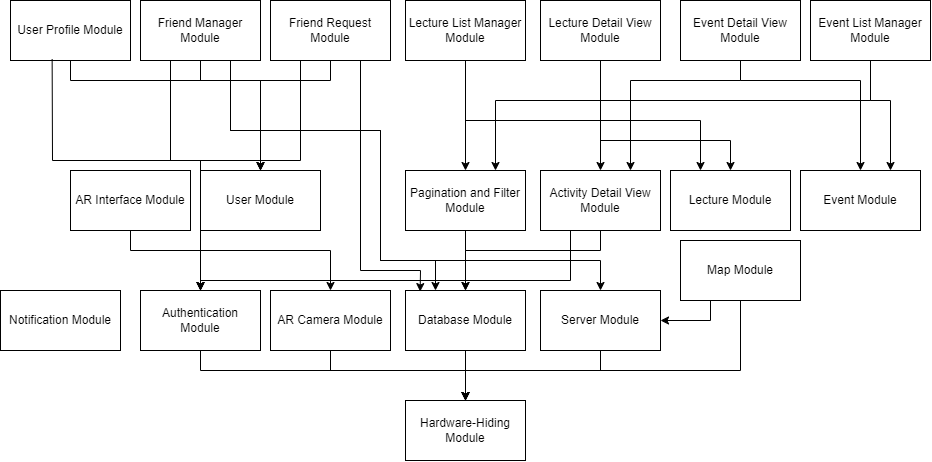
\includegraphics[width=0.7\textwidth]{UsesHierarchy.png}
\caption{Use hierarchy among modules}
\label{FigUH}
\end{figure}

\section{Timeline}
\begin{table}[H]
\centering
\begin{tabular}{p{0.35\textwidth} p{0.3\textwidth}  p{0.3\textwidth}}
\toprule
Module Name & Team Member & Due Date \\
\midrule
Database & Zihao Du & Dec. 4, 2023\\
User & Zihao Du & Nov 15, 2023\\
Friend Manager & Zihao Du & Jan 15, 2024\\
Notification & Zihao Du & Feb 5th, 2024\\
\bottomrule
\end{tabular}
\caption{CampusConnections Module Completion Timeline}
\end{table}

\newpage{}

\appendix

\section{Reflection}

The information in this section will be used to evaluate the team members on the
graduate attribute of Problem Analysis and Design.  Please answer the following questions:

\begin{enumerate}
  \item What are the limitations of your solution?  Put another way, given
  unlimited resources, what could you do to make the project better? (LO\_ProbSolutions)
  \item Give a brief overview of other design solutions you considered.  What
  are the benefits and tradeoffs of those other designs compared with the chosen
  design?  From all the potential options, why did you select documented design?
  (LO\_Explores)
\end{enumerate}

\newpage
\bibliographystyle {plainnat}
\bibliography{../../../refs/References}

\newpage{}

\end{document}